\documentclass[10pt]{article}
\renewcommand{\familydefault}{cmss}

\newcommand{\rp}{\textbf{Raspberry Pi}\xspace}

\usepackage{xspace}
\usepackage[ngerman]{babel} % this is needed for umlauts
\usepackage[utf8]{inputenc} % this is needed for umlauts
\usepackage[T1]{fontenc} % this is needed for correct output of umlauts in pdf
\usepackage[pdftex,breaklinks,colorlinks,
citecolor=blue,
urlcolor=blue,
pdftitle={Lecture 9},
pdfauthor={Ryan Higginbottom},
pdfsubject={LaTeX}]{hyperref}
\usepackage{graphicx}
\graphicspath{ {img/} }
\DeclareGraphicsExtensions{.jpg}

\begin{document}
\title{Raspberry Pi}
\maketitle

Die \rp Hardware ist ein Einplatinen Computer der von der britischen \href{https://www.raspberrypi.org/}{Raspberry Pi Foundation} gefertigt wird.

Der \rp wurde 2008 ursprünglich entwickelt, Kinder spielerisch in die Welt der Programmierung \& Elektronik einzuführen. Jedoch führte die einfache Handhabung und die fast unendlichen Möglichkeiten zu einer grossen Community, die mittlerweile durch alle Schichten und Altersklassen geht.

Der Name wird wie \textit{raspberry pie} ausgesprochen, das englische Wort für Himbeerkuchen. Die \textit{Himbeere} knüpft an die Tradition an, Computer nach Früchten zu benennen, wie etwa \textbf{Apple}. Das \textbf{Pi} stammt aus \textit{Python}, einer Programmiersprache.

Bis Februar 2017 wurden mehr als zwölf Millionen Geräte verkauft. Die Entwicklung des \textbf{Raspberry Pi} wurde mit mehreren Auszeichnungen bzw. Ehrungen bedacht. Es existiert ein großes Zubehör- und Softwareangebot für zahlreiche Anwendungsbereiche. Verbreitet ist beispielsweise die Verwendung als \href{https://www.youtube.com/watch?v=YPu7oSVbMVo}{Mediacenter}, da der Rechner Videodaten mit voller HD-Auflösung (1080p) dekodieren und über die HDMI-Schnittstelle ausgeben kann. 

\section{Anschlüsse und Komponenten}

Bevor man mit dem \rp richtig loslegen kann, muss man zumindest grob wissen, wo welche Anschlüsse und Komponenten liegen und für was sie gut sind. Deshalb gilt es, alle wichtigen Anschlüsse und Bauteile des \rp richtig zu identifizieren.

\subsection{Aufgabe}

Auf dem unteren Foto des \rp zeichne die folgenden Anschlüsse und Komponenten ein.

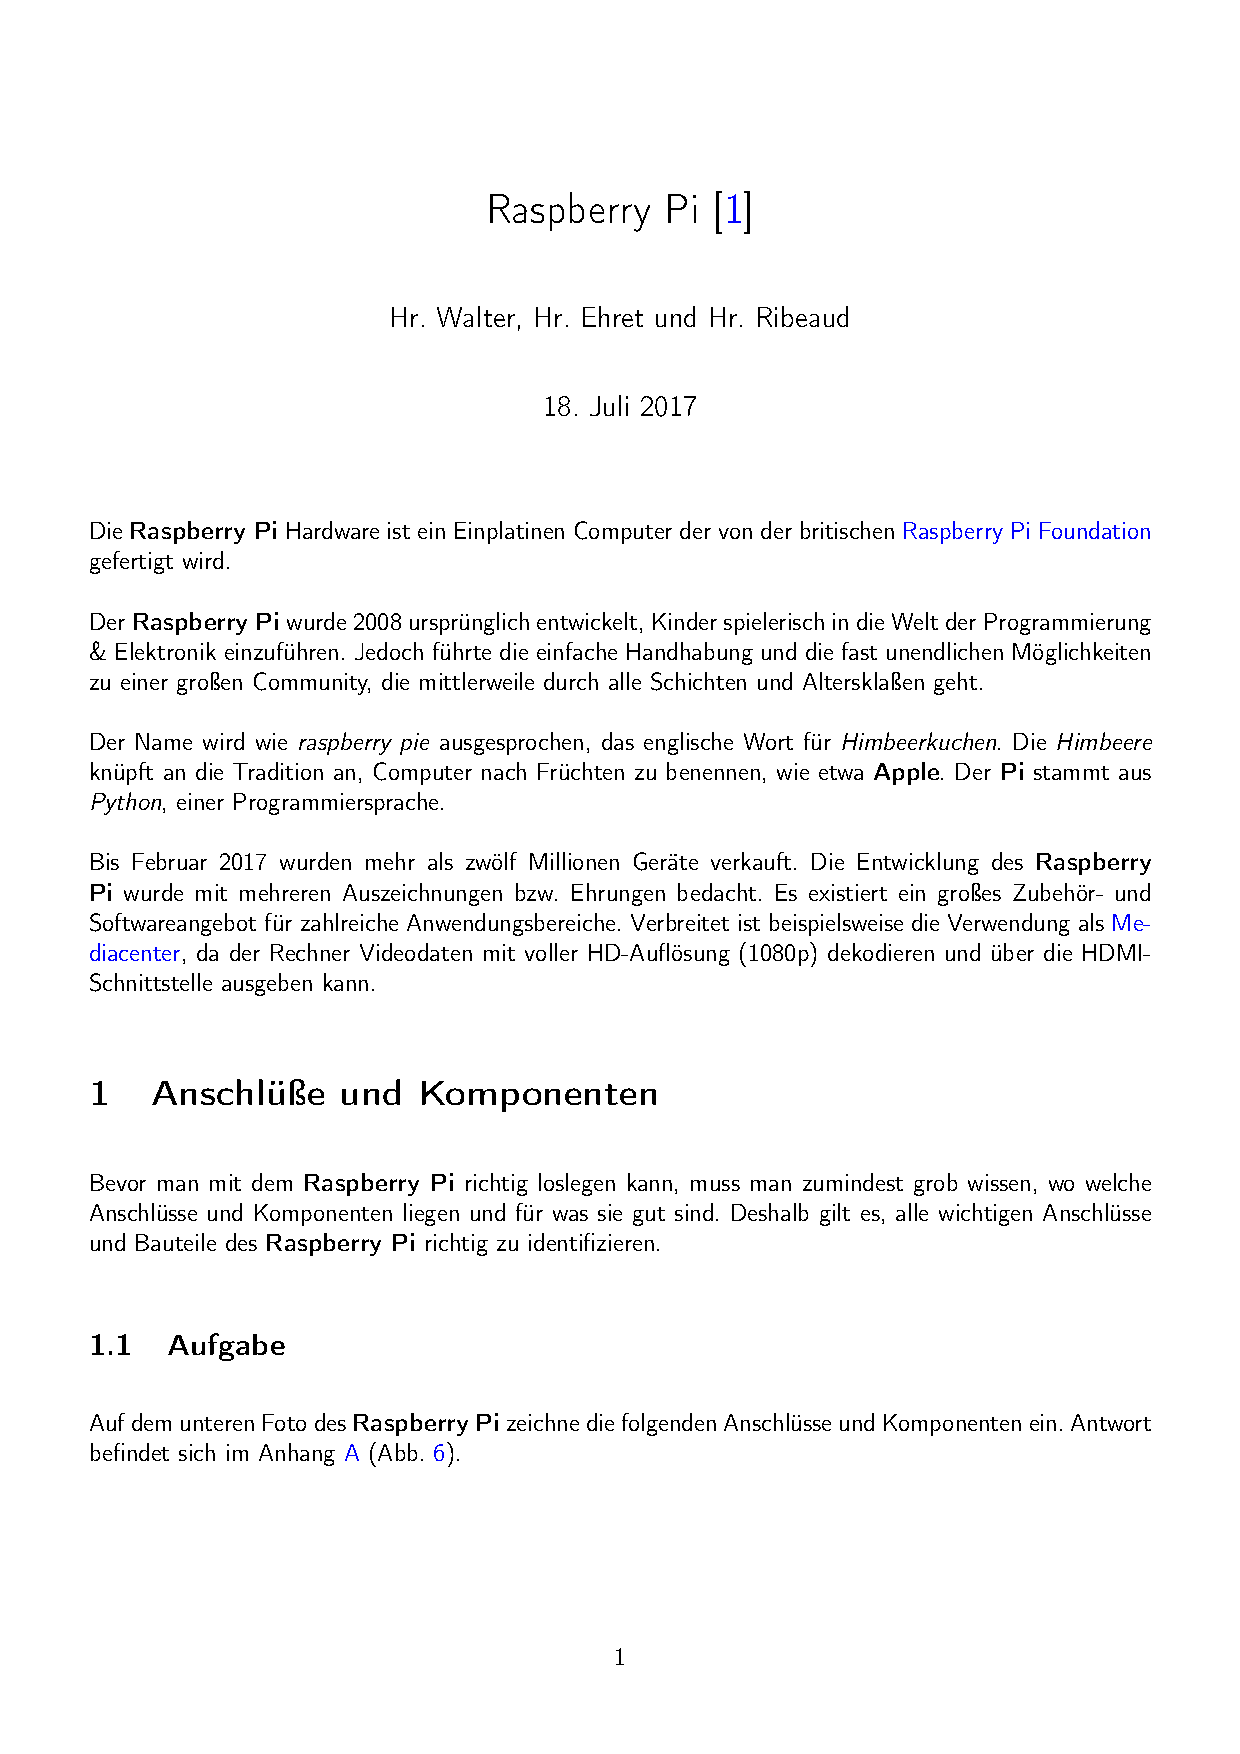
\includegraphics[scale=1.1]{raspberry}

\begin{enumerate}
\item Wo befindet sich der Tastatur- und Maus-Anschluss (USB)?
\item Wo befindet sich der Netzwerk-Anschluss (Ethernet)?
\item Wo befindet sich der Anschluss für einen Bildschirm (HDMI)?
\item Wo befindet sich der Anschluss für Lautsprecher (Klinke)?
\item Wo befindet sich der Anschluss für die Energieversorgung (Micro-USB)?
\item Wo befindet sich der Steckplatz für die SD-Speicherkarte?
\item Wo befindet sich der Steckplatz für Erweiterungen (GPIO)?
\end{enumerate}

\appendix
\makeatletter
\def\@seccntformat#1{Appendix~\csname the#1\endcsname:\quad}
\makeatother

\section{First appendix}

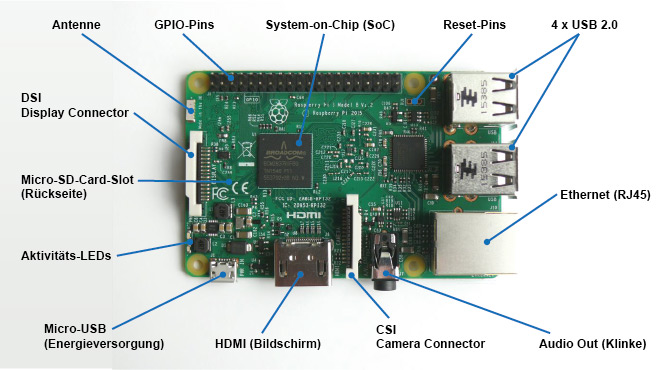
\includegraphics[scale=0.5]{raspberry_loesung}

\end{document}
